% Shared standalone design for the editable figure reconstructions.
\documentclass[tikz,border=5pt,10pt]{standalone}
\usepackage[T1]{fontenc}
\usepackage[utf8]{inputenc}
\usepackage{newpxtext,newpxmath}
\usepackage[scaled=.94]{sourcesanspro}
\usepackage{pgfplots}
\pgfplotsset{compat=1.18}
\usetikzlibrary{arrows.meta,calc,positioning,decorations.pathreplacing,
  decorations.markings,patterns,matrix,shapes.geometric,fit,backgrounds,
  intersections,angles,quotes}
\definecolor{ink}{HTML}{203746}
\definecolor{accent}{HTML}{146C78}
\definecolor{muted}{HTML}{667780}
\definecolor{signalred}{HTML}{B94B44}
\color{ink}
\tikzset{>=Latex,line width=.8pt,
  every node/.style={font=\small},
  axis/.style={->,draw=muted,line width=.5pt},
  guide/.style={draw=muted,dashed,line width=.45pt},
  curve/.style={draw=accent,line width=1pt},
  marker/.style={circle,fill=accent,inner sep=1.5pt},
  labelbox/.style={fill=white,inner sep=2pt}}

\begin{document}
\begin{tikzpicture}
\node at (5.4,3.65) {$b_{\lambda,\beta}(\sigma)=\dfrac{\lambda\sigma^\beta}{\lambda+\sigma^2},\qquad D_{\lambda,\beta}=\sup_{\sigma\geq0}b_{\lambda,\beta}(\sigma)$};
\foreach \s/\title in {0/{$0<\beta<2$},4.05/{$\beta=2$},8.1/{$\beta>2$}}{
\begin{scope}[shift={(\s,0)}]\draw[axis](0,0)--(3.3,0)node[right]{$\sigma$};\draw[axis](0,0)--(0,2.65);\node[font=\small\sffamily]at(1.5,2.9){\title};\end{scope}}
\draw[curve]plot[domain=0:3,samples=80](\x,{4*\x/(1+\x*\x)});
\draw[guide](0,2)node[left]{$D_{\lambda,\beta}$}--(1,2)--(1,0);\fill[accent](1,2)circle(1.5pt);
\node[align=center]at(1.4,-.7){$\displaystyle\sigma_* = \sqrt{\frac{\beta\lambda}{2-\beta}}$};
\begin{scope}[shift={(4.05,0)}]
\draw[curve]plot[domain=0:3,samples=80](\x,{2.3*\x*\x/(.5+\x*\x)});
\draw[guide](0,2.3)node[left]{$\lambda$}--(3.05,2.3);
\node at(1.5,-.7){$D_{\lambda,2}=\lambda$};
\end{scope}
\begin{scope}[shift={(8.1,0)}]
\draw[curve,->]plot[domain=0:3,samples=80](\x,{.8*\x*\x*\x/(1+\x*\x)});
\node at(1.5,-.7){$D_{\lambda,\beta}=+\infty$};
\end{scope}
\node[align=center,text width=11.8cm,font=\footnotesize]at(5.4,-1.7){Here \mbox{$\lambda>0$} and the supremum ranges over all \mbox{$\sigma\geq0$}.\\On a fixed bounded operator, only \mbox{$0\leq\sigma\leq\|\Phi\|$} is relevant.};
\end{tikzpicture}
\end{document}
